\chapter{Project}
%\label{chapter:title}
\section{The technological context}

The idea of processing in memory is an old one and has been considered since the mid 1990s~\cite{stone1970logic, Kautz1969, shaw1981non, kogge1994, gokhale1995processing, patterson1997case, oskin1998active, kang1999flexram, Mai:2000:SMM:339647.339673, Draper:2002:ADP:514191.514197,aga.hpca17,eckert2018neural,fujiki2019duality,kang.icassp14,seshadri.micro17,seshadri2013rowclone,angizi2019graphide,kim.hpca18,kim.hpca19,gao2020computedram,chang.hpca16,xin2020elp2im,li.micro17,deng.dac2018,hajinazarsimdram,rezaei2020nom,wang2020figaro,ali2019memory,li.dac16,angizi2018pima,angizi2018cmp,angizi2019dna,levy.microelec14,kvatinsky.tcasii14,shafiee2016isaac,kvatinsky.iccd11,kvatinsky.tvlsi14,gaillardon2016plim,bhattacharjee2017revamp,hamdioui2015memristor,xie2015fast,hamdioui2017myth,yu2018memristive,syncron,fernandez2020natsa,cali2020genasm,kim.bmc18,ahn.pei.isca15,ahn.tesseract.isca15,boroumand.asplos18,boroumand2019conda,singh2019napel,asghari-moghaddam.micro16,DBLP:conf/sigmod/BabarinsaI15,chi2016prime,farmahini2015nda,gao.pact15,DBLP:conf/hpca/GaoK16,gu.isca16,guo2014wondp,hashemi.isca16,cont-runahead,hsieh.isca16,kim.isca16,kim.sc17,DBLP:conf/IEEEpact/LeeSK15,liu-spaa17,morad.taco15,nai2017graphpim,pattnaik.pact16,pugsley2014ndc,zhang.hpdc14,zhu2013accelerating,DBLP:conf/isca/AkinFH15,gao2017tetris,drumond2017mondrian,dai2018graphh,zhang2018graphp,huang2020heterogeneous,zhuo2019graphq,santos2017operand,ghoseibm2019,wen2017rebooting,besta2021sisa,ferreira2021pluto,olgun2021quactrng,lloyd2015memory,elliott1999computational,zheng2016tcam,landgraf2021combining,rodrigues2016scattergather,lloyd2018dse,lloyd2017keyvalue,gokhale2015rearr,nair2015active,jacob2016compiling,sura2015data,nair2015evolution,balasubramonian2014near,xi2020memory}.
Despite being the first company to reach the stage of a commercially available PIM product, UPMEM is in need of more technological demonstrators to encourage widespread adoption of its system.

My role during this apprenticeship was to develop machine-learning applications running on PIM that display an enticing performance gain (be it speed or energy consumption) when compared to existing CPU or GPU implementations.

\subsection{Motivation}

Data transfer on SDRAM is limited by a communication bus. Currently, the transfer rate on DDR5-6400 is 51.2 GB/s per channel (409.6 GB/s on an 8-channel system). Although this speed has been steadily increasing, there are popular algorithms today that end up with memory-bound performances (such as pooling operations in neural networks~\cite{nvidia.memory2020}).

The principle of PIM is to execute as many operations as possible in memory, and to minimize the number of operations that are executed in the CPU, thus limiting the flow of data through the memory bus.

\subsection{Architecture}

UPMEM DIMM is based on DDR4 and attaches an onboard RISC-V processor to each 64 MB memory bank, these processors are called DPU for Data Processing Units. A schematic representation of an UPMEM DIMM can be seen in Figure \ref{fig:DIMM}. The DPUs access their MRAM via a DMA engine. The transfer rate between each DPU and its associated memory bank (called MRAM) is 1 GB/s. This means that on a server with the maximum number of DPUs (2560), the total transfer rate is 2.5 TB/s. Each DPU can execute up to 24 tasklets in parallel.

\begin{figure}[htb]
    \centering
    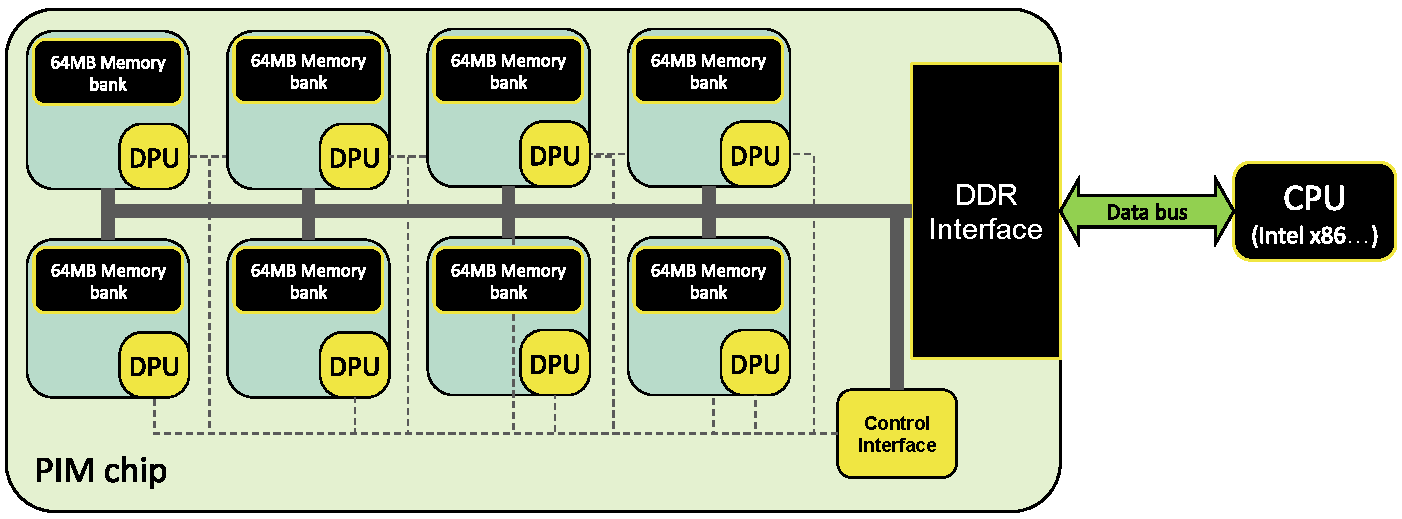
\includegraphics[width=0.95\linewidth]{figures/PIM.pdf}
    \caption{\label{fig:DIMM}UPMEM PIM Architecture}
\end{figure}

Each DIMM has two ranks with 64 DPUs each. This amounts to 8.2 GB of memory per DIMM. Each DPU also has an internal Work RAM (WRAM) of 64 KB.

In reality, at the hardware level, DPUs come in pairs, and each pair is connected to a memory bank. However, this is entirely transparent to the programmer. Therefore, we will ignore this fact.

\subsection{Limitations and Constraints}
\label{subsection:Limitations}

A number of engineering choices had to be made to make UPMEM PIM a viable product. We will now list the ones that are most relevant to developers:

\begin{itemize}
    \item \textbf{Floating point arithmetic:} Due to the limited space available on the chip, the DPUs do not have a floating point unit, and therefore do not support floating point operations at the hardware level. It is still possible to perform floating point operations on the DPUs, but these are simulated operations, and therefore much slower than hardware supported operations. For example, a single 32-bit floating point multiplication on a DPU will take upwards of 120 instructions.
    \item \textbf{Discrete arithmetic:} At the hardware level, the DPUs support 32 bits integer additions/subtractions, and 8 bits integer multiplications.
    \item \textbf{CPU-DPU concurrency:} The memory banks cannot be accessed by the DPUs and host CPU at the same time. Therefore, the DPUs cannot be running while the host CPU is reading results from the memory banks. This prevents any kind of streaming programming model. Instead, iterations must be performed between host and PIM.
    \item \textbf{Data parallelism:} The DPUs cannot communicate with each other. The orchestration must be performed by the host CPU. Since every CPU-DPU communication is relatively costly, implemented algorithms must be data-parallel.
    \item \textbf{Thread parallelism:} Being RISC processors, the DPUs need to execute instructions in parallel to take full advantage of the available resources. Instructions in a DPU go through a pipeline of 11 stages when they execute. Thus, we need to use at least 11 tasklets to reach peak performance. In practice, we generally use 16 tasklets because it's a power of two, and because the extra tasklets can sometimes hide the latency of DMA accesses. Tasklets can synchronize via mutexes or semaphores, but this has a performance cost and should be kept to a minimum.
    \item \textbf{Stack size:} Each DPU has to share its WRAM between its tasklets, and generally keep some space for global variables. This usually leaves 1 KB or 2 KB of stack for each tasklet.
    \item \textbf{DMA memory accesses:} Accessing the MRAM is slower than the WRAM, and it incurs some overhead. Therefore, MRAM accesses should be done in large blocks, or streamed with a sequential reader. Performing too many random accesses impacts performance negatively. Also, there are alignment constraints: each memory access has to be aligned on 8 bytes. Forgetting that fact can lead to concurrency issues if two tasklets try to modify two values in the same 8-byte aligned memory location.
    \item \textbf{Compilation:} The DPU kernels are compiled with a modified version of the LLVM compiler. While it does generally perform as expected, the C standard was mostly created with x86 and x86\_64 processors in mind. This means that sometimes the compiler will generate code that is not optimized for the target architecture. An example of that behavior can be seen in section \ref{annex:promotion}.
\end{itemize}

\section{Algorithms}

Here we will present the machine learning algorithms that we chose to implement in UPMEM PIM. Both those algorithms are implemented in Scikit-learn~\cite{pedregosa2011scikit} and RAPIDS~\cite{rapids}, allowing us to run benchmarks against CPU and GPU.

\subsection{K-Means}

\begin{wrapfigure}{L}{0.45\textwidth}
    \centering
    \resizebox{0.3\textwidth}{!}{
        \begin{tikzpicture}[node distance=2cm]
            \begin{scope}
                \node (kcpupro1c) [processcpu] {For each point find the nearest centroid};
                \node (kcpupro2c) [processcpu, below=\vspacing of kcpupro1c] {Sum the features of all points in each cluster};
                \node (kcpupro3c) [processcpu, below=\vspacing of kcpupro2c] {Average the new centroids of clusters};
                \node (kcpudec1) [decision, below=\vspacing of kcpupro3c] {Centroids changed?};
                \node (kcpuout1) [stop, below=\vspacing of kcpudec1] {Output centroids};

                \draw [arrow] (kcpupro1c) -- (kcpupro2c);
                \draw [arrow] (kcpupro2c) -- (kcpupro3c);
                \draw [arrow] (kcpupro3c) -- (kcpudec1);
                \draw [arrow] (kcpudec1) -- node[anchor=east] {no} (kcpuout1);
                \draw [arrow] (kcpudec1.east) -- node[anchor=south] {yes} ++(2,0) |- (kcpupro1c.east);
            \end{scope}
        \end{tikzpicture}
    }
    \caption{\label{fig:KMeansCPU}The K-Means algorithm on CPU}
\end{wrapfigure}

K-means~\cite{Lloyd82leastsquares} is a popular clustering algorithm, due to its simplicity and efficiency. It is used to identify unlabeled groups in a dataset, by grouping them in clusters around a so-called centroid. The algorithm is divided into an E (for Evaluation) phase, where the points in the dataset are assigned to the closest centroid, and an M (for Move) phase, where the centroids are recalculated as the average of the points in their cluster. A simplified flowchart of the algorithm can be seen in Figure \ref{fig:KMeansCPU}.

This natural division of the K-Means suits the UPMEM architecture, as the E step can be entirely performed in memory, and the M step can be performed when the CPU and DPUs synchronize.

It should be noted that there exists several variants of the K-Means algorithm, such as the Elkan variant~\cite{elkan2003using} which uses the triangle inequality to reduce the amount of distances calculations that have to be performed. For our implementation and for comparisons, we stuck with the original Lloyd variant. There are two reasons for that:
\begin{itemize}
    \item It is the simplest to implement.
    \item When it comes to the Scikit-learn implementation, it turns out in most benchmarks that the Elkan variant is slower. This boils down to implementation. The core of the Lloyd algorithm is essentially a large matrix multiplication. The Scikit-learn implementation takes full advantage of that fact by making a direct call to the Intel MKL~\cite{mkl} to perform that multiplication. Being developed by Intel, the MKL uses the vectorization capabilities built in x86 processors to speed up the computation. By contrast, the Elkan variant is implemented with naive loops, and puts the onus of optimization on the compiler, which cannot reach the same performances. It should be noted that Intel also only implemented the Lloyd algorithm in their own Data Analytics Library.
\end{itemize}
Since we are trying to compare hardware capabilities, it is better to stick to the Lloyd variant.

A point should be made about the norm used to compute distances. Since performing multiplications on DPUs is slow, it could be tempting to use the L1 norm instead of the Euclidean L2 norm. However, a naive approach consisting of simply replacing the L2 distances with L1 distances in K-Means would not converge in the general case~\cite{bradley1996clustering}. The reason is that K-Means is a variance-minimizing algorithm, and the mean is the minimizer of the variance. The minimizer of the L1-variance is the median. Thus, if we wanted to avoid multiplications altogether, we should implement the K-Medians~\cite{jain1988algorithms} algorithm. While it is possible in principle, it would require using a median-of-median approach~\cite{blum1973time}, and implementing it on PIM while limiting CPU-DPU communication would be much more challenging.

\subsection{Decision Trees}

\begin{wrapfigure}{R}{0.4\textwidth}
    \centering
    \resizebox{0.3\textwidth}{!}{
        \begin{tikzpicture}[node distance=2cm]
            \begin{scope}
                \node (pro1c) [io] {Load an active leaf};
                \node (pro2c) [processcpu, below=\vspacing of pro1c] {Evaluate splits};
                \node (pro3c) [processcpu, below=\vspacing of pro2c] {Commit best split};
                \node (pro52c) [processcpu, below=\vspacing of pro3c] {create new leaves};
                \node (pro6c) [decision, below=\vspacing of pro52c] {Tree finished?};
                \node (out1) [stop, below=\vspacing of pro6c] {Output Tree};

                \draw [arrow] (pro1c) -- (pro2c);
                \draw [arrow] (pro2c) -- (pro3c);
                \draw [arrow] (pro3c) -- (pro52c);
                \draw [arrow] (pro52c) -- (pro6c);
                \draw [arrow] (pro6c) -- node[anchor=east] {yes} (out1);
                \draw [arrow] (pro6c.east) -- node[anchor=south] {no} ++(2,0) |- (pro1c.east);
            \end{scope}
        \end{tikzpicture}
    }
    \caption{\label{fig:TreeCPU}A tree algorithm on CPU}
\end{wrapfigure}


Decision trees~\cite{suthaharan2016decision} are tree-based algorithms used for classification and regression, commonly known as CART (for Classification And Regression Trees). They successively partition the dataset based on thresholds. A simplified representation of a tree-building algorithm can be seen in Figure \ref{fig:TreeCPU}. Trees are a good candidate for PIM because the amount of calculations is limited, and most of the workload is about memory reads and writes.

In this work, we only implemented classification trees, as this allows us to avoid any sort of floating-point operations on the DPUs, other than comparisons. Furthermore, we only implemented the so-called \emph{extremely randomized tree}~\cite{geurts2006extremely}, referred to as \emph{extra-tree} in Scikit-learn. Unlike the regular trees, this variant of the algorithm only selects thresholds at random, and does not use any heuristic to select the best threshold. This allows us to make the CPU "forget" about the dataset once it has been loaded into the DIMMs. Extremely randomized tree present a larger bias and lower variance than regular trees, and are commonly used as the base unit for forests of randomized trees~\cite{breiman2001random}.

\section{Collaboration}

Once the potential of machine learning algorithms in PIM started to become apparent, we decided to start a collaboration with Juan Gómez Luna of ETH Zürich and his student Yuxin Guo.

Dr. Gómez Luna provided us with the academic insights on what the scope of a publication on machine learning in-memory should be. He also wrote the bulk of our joint article. Meanwhile, Yuxin Guo implemented the Linear Regression and Logistic Regression algorithms in UPMEM PIM. I won't expand on the result of his work in his report, but they can be found in the soon-to-be-published article.

\section{Work Organization}

Internally, the software team has two weekly stand-ups on Monday and Wednesday, and one software point on Friday. The stand-ups are meant to update the rest of the team on the current advancement of projects, and the point is to discuss the projects at more length.
There is also a company-wide stand-up on Tuesday, where department heads update everyone on their advancement.
This project also had weekly synchronization meetings with the ETH Zürich team, where we discussed necessary additions to the article.

For most of the work, the experiment results were shared with the ETH team in Google Sheets, however I've now set up a data version control system with DVC~\cite{ruslan_kuprieiev_2022_6501662} to track the experiments.

\section{Deliverables}

\subsection{Python Libraries}

My first task at my arrival at UPMEM was to work on an existing C code for K-Means that had been provided by an academic partner, and suffered from extremely poor optimization (about 1000 times slower than a CPU code). As part of my work on the code, I decided to reimplement it as a Python library. The main motivation here being that if we want to garner interest among data scientists for UPMEM PIM, there should be a Python API. The library is available on UPMEM GitHub repository. It uses C code for the backend, and Pybind-11 for the Python bindings.

Decision trees are also available as a Python library. In an effort of fairness, most of the backend code is written in Cython, to mimic the Scikit-learn implementation.

For now the two libraries are separate, but they will be merged, along with Linear Regression and Logistic Regression, in a yet-to-be-named PIM ML library.

\subsection{Benchmarks}

With the co-publication in mind, a lot of effort was put into benchmarking the algorithms. This required implementing various performance counter, as well as modifying parts of Scikit-learn to add those same performance counters. We decided not to use native Python profiling tools for this task, because they have a significant overhead and shouldn't be used for benchmarking, as stated in the Python documentation~\cite{10.5555/1593511}.

\subsection{Compiler Simulation}

Apart from generating interest, the applications team role is also to inform the hardware team about which improvements to the future versions of the DPUs would result in the best performance gains. In this optic, I tested different versions of the K-Means on the DPU software simulator, with simulated assembly instructions, and compared the resulting instructions counts.
